\section{Multi-Layered Perceptrons} 

  We build upon what we already know: generalized linear models. In simple regression, we transform the inputs into the relevant features $\mathbf{x}_n \mapsto \boldsymbol{\phi} (\mathbf{x}_n) = \boldsymbol{\phi}_n$ and then, when we construct a generalized linear model, we assume that the conditional distribution $Y \mid X = x$ is in the canonical exponential family, with some natural parameter $\eta(x)$ and expected mean $\mu(x) = \mathbb{E}[Y \mid X = x]$. Then, to choose the link function $g$ that related $g(\mu(x)) = x^T \beta$, we can set it to be the canonical link $g$ that maps $\mu$ to $\eta$. That is, we have $g(\mu(x)) = x^T \beta = \eta (x)$ such that the natural parameter is linearly dependent on the input. The inverse $g^{-1}$ of the link function is called the \textbf{activation function}, which connects the expected mean to a linear function of $x$. 
  \begin{equation}
    h_\beta (x) = g^{-1} (x^T \beta) = \mu(x) = \mathbb{E}[Y \mid X = x]
  \end{equation}
  Now, note that for a classification problem, the decision boundary defined in the $\boldsymbol{\phi}$ feature space is linear, but it may not be linear in the input space $\mathcal{X}$. We would like to extend this model by making the basis functions $\boldsymbol{\phi}_n$ depend on the parameters $\mathbf{w}$ and then allow these parameters to be adjusted during training. 

  \begin{figure}[H]
    \centering
    \begin{subfigure}[t]{0.24\textwidth}
      \centering
      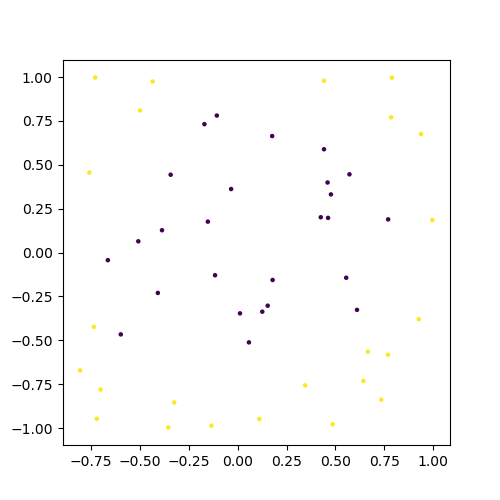
\includegraphics[width=\textwidth]{img/untrans_data.png}
      \caption{Data in space $\mathcal{X} = \mathbb{R}^2$.}
      \label{fig:raw_points}
    \end{subfigure}
    \hfill
    \begin{subfigure}[t]{0.24\textwidth}
      \centering
      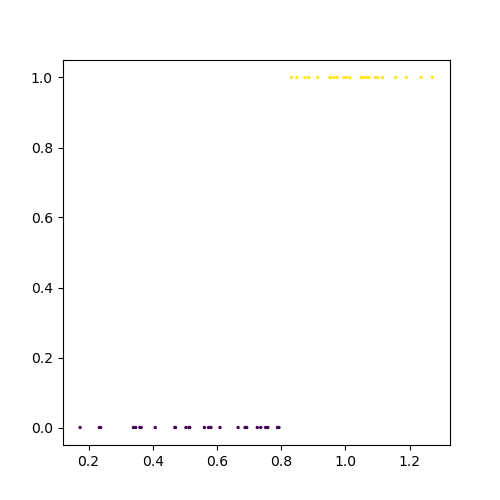
\includegraphics[width=\textwidth]{img/trans_data.png}
      \caption{Transformed data $\phi(\mathbf{x}) = \|\mathbf{x}\|$.}
      \label{fig:transformed_points}
    \end{subfigure}
    \hfill
    \begin{subfigure}[t]{0.24\textwidth}
      \centering
      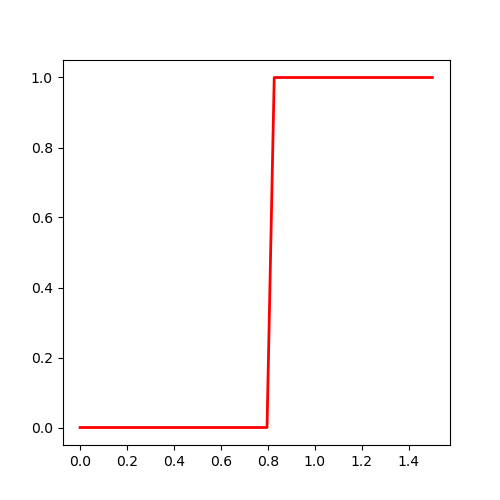
\includegraphics[width=\textwidth]{img/trans_fit.png}
      \caption{Logistic fit in transformed space.}
      \label{fig:transformed_trained}
    \end{subfigure}
    \hfill
    \begin{subfigure}[t]{0.24\textwidth}
      \centering
      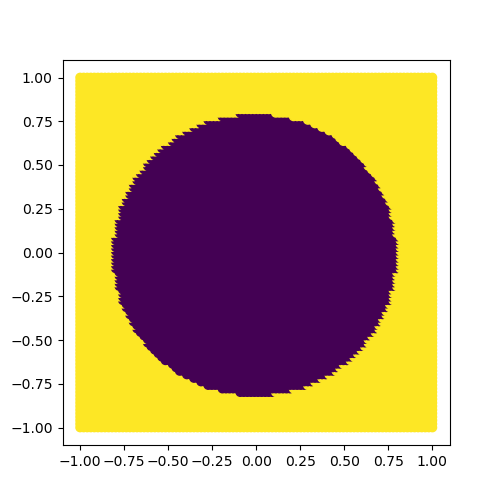
\includegraphics[width=\textwidth]{img/untrans_fit.png}
      \caption{Logistic fit to data in input space.}
      \label{fig:raw_trained}
    \end{subfigure}
    \caption{Consider the set of points in $\mathbb{R}^2$ with the corresponding class. We transform the features to $\boldsymbol{\phi}(x_1, x_2) = x_1^2 + x_2^2$, which gives us a new space to work with. Fitting logistic regression onto this gives a linear decision boundary in the space $\boldsymbol{\phi}$, but the boundary is circular in $\mathcal{X} = \mathbb{R}^2$.}
    \label{fig:logistic_transformed}
  \end{figure}

\subsection{Feedforward Fully-Connected Networks}

  So how should we construct parametric nonlinear basis functions? One way is to have a similar architecture as GLMs by having a linear map followed by an activation function $f(x) = \sigma(w^T x + b)$. The simplest such function with the activation function as the step function 
  \begin{equation}
    f(z) = \begin{cases} 1 & \text{ if } z \geq 0 \\ 0 & \text{ if } z < 0 \end{cases}
  \end{equation}
  is the perceptron algorithm. It divides $\mathbb{R}^d$ using a hyperplane $\boldsymbol{\omega}^T \mathbf{x} + b = 0$ and linearly classifies all points on one side to value $1$ and the other side to value $0$. This is similar to a neuron, which takes in a value and outputs a ``signal" if the function evaluated gets past a threshold. However, for reasons regarding training these networks, we would like to use smooth activation functions for this, so we would use different activations. Hence we have a neuron. 

  \begin{definition}[Neuron]
    A \textbf{neuron} is a function of form 
    \begin{equation}
      y = \sigma(\mathbf{w}^T x  + b)
    \end{equation}
    where $\sigma: \mathbb{R} \rightarrow \mathbb{R}$ is any nonlinear function, called an \textbf{activation functions}. 
  \end{definition}
  
  Ultimately, a neural net is really just a generalized linear model with some trained feature extractors, which is why in practice, if researchers want to predict a smaller dataset, they take a pretrained model on a related larger dataset and simply tune the final layer, since the second last layer most likely encodes all the relevant features. This is called \textit{transfer learning}. But historically, it was called a \textit{multilayer perceptron} and the name stuck. 

  \begin{definition}[Feedforward, Fully-Connected Multilayer Perceptron]
    A $L$-layer \textbf{multilayer perceptron (MLP)} $f_\theta : \mathbb{R}^D \rightarrow \mathbb{R}^M$, with parameters $\theta$, is a function of form 
    \begin{equation}
      h_\theta (\mathbf{x}) \coloneqq \sigma^{[L]} \circ W^{[L]} \circ \sigma^{[L-1]} \circ W^{[L-1]} \circ \cdots \circ \sigma^{[1]} \circ W^{[1]} (\mathbf{x})
    \end{equation}
    where $\sigma^{[l]}: \mathbb{R}^{N^{[l]}} \rightarrow \mathbb{R}^{N^{[l]}}$ is an activation function and $W^{[l]}: \mathbb{R}^{N^{[l-1]}} \rightarrow \mathbb{R}^{N^{[l]}}$ is an affine map. We will use the following notation. 
    \begin{enumerate}
      \item The inputs will be labeled $\mathbf{x} = a^{[0]}$ which is in $\mathbb{R}^{N^{[0]}} = \mathbb{R}^D$. 
      
      \item We map $a^{[l]} \in \mathbb{R}^{N^{[l]}} \mapsto W^{[l+1]} a^{[l]} + b^{[l+1]}= z^{[l+1]} \in \mathbb{R}^{N^{[l+1]}}$, where $z$ denotes a vector after an affine transformation. 

      \item We map $z^{[l+1]} \in \mathbb{R}^{N^{[l+1]}} \mapsto \sigma(z^{[l+1]}) = a^{[l+1]} \in \mathbb{R}^{N^{[l+1]}}$, where $a$ denotes a vector after an activation function. 

      \item We keep doing this until we reach the second last layer with vector $a^{[L-1]}$. Note that in the last layer we do \textit{not} apply an activation function. 
    \end{enumerate}

    \begin{figure}[H]
      \centering 
      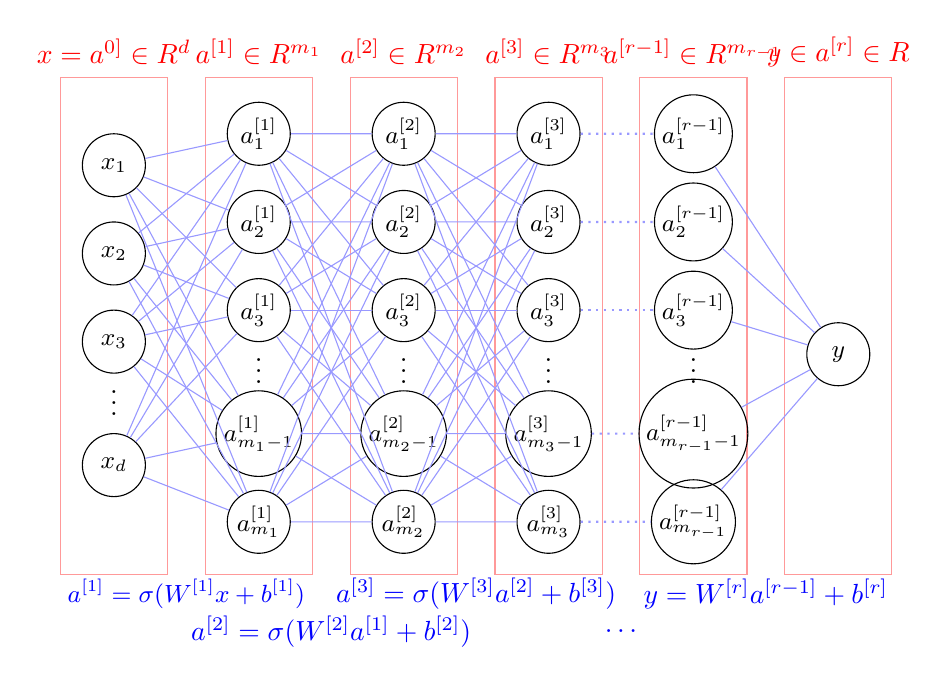
\begin{tikzpicture}[
        scale=0.8, 
        node distance=2cm,
        neuron/.style={circle, draw, minimum size=0.8cm, inner sep=1pt, font=\small},
        annotation/.style={text width=3cm},
        >=latex
      ]
        % Define some variables for consistent spacing
        \def\layersep{2.3}
        \def\neuronsep{1.4}
        \def\boxwidth{1.7}
        \def\boxheight{8}
        
        % Add dimension annotations above boxes in red
        \node[red] at (0, \boxheight/2 + 0.8) {$x = a^{0]} \in \mathbb{R}^d$};
        \node[red] at (\layersep, \boxheight/2 + 0.8) {$a^{[1]} \in \mathbb{R}^{m_1}$};
        \node[red] at (2*\layersep, \boxheight/2 + 0.8) {$a^{[2]} \in \mathbb{R}^{m_2}$};
        \node[red] at (3*\layersep, \boxheight/2 + 0.8) {$a^{[3]} \in \mathbb{R}^{m_3}$};
        \node[red] at (4*\layersep, \boxheight/2 + 0.8) {$a^{[r-1]} \in \mathbb{R}^{m_{r-1}}$};
        \node[red] at (5*\layersep, \boxheight/2 + 0.8) {$y \in a^{[r]} \in \mathbb{R}$};
        
        % Draw boxes
        \foreach \x in {0,1,2,3,4,5} {
            \draw[red!40] (\x*\layersep-\boxwidth/2, -\boxheight/2 + 0.5) rectangle (\x*\layersep+\boxwidth/2, \boxheight/2 + 0.4);
        }
        
        % Input layer (x) with adjusted vertical spacing
        \node[neuron] (x1) at (0, 3) {$x_1$};
        \node[neuron] (x2) at (0, {3-\neuronsep}) {$x_2$};
        \node[neuron] (x3) at (0, {3-2*\neuronsep}) {$x_3$};
        \node at (0, {3-2.6*\neuronsep}) {$\vdots$};
        \node[neuron] (xd) at (0, {3-3.4*\neuronsep}) {$x_d$};
        
        % Hidden layers with matching spacing pattern
        \foreach \l in {1,2,3} {
            \node[neuron] (a\l1) at (\l*\layersep, 3.5) {$a^{[\l]}_1$};
            \node[neuron] (a\l2) at (\l*\layersep, {3.5-\neuronsep}) {$a^{[\l]}_2$};
            \node[neuron] (a\l3) at (\l*\layersep, {3.5-2*\neuronsep}) {$a^{[\l]}_3$};
            \node at (\l*\layersep, {3.5-2.6*\neuronsep}) {$\vdots$};
            \node[neuron] (a\l m1) at (\l*\layersep, {3.5-3.4*\neuronsep}) {$a^{[\l]}_{m_{\l}-1}$};
            \node[neuron] (a\l m) at (\l*\layersep, {3.5-4.4*\neuronsep}) {$a^{[\l]}_{m_{\l}}$};
        }
        
        % Second-to-last layer (r-1)
        \node[neuron] (ar1) at (4*\layersep, 3.5) {$a^{[r-1]}_1$};
        \node[neuron] (ar2) at (4*\layersep, {3.5-\neuronsep}) {$a^{[r-1]}_2$};
        \node[neuron] (ar3) at (4*\layersep, {3.5-2*\neuronsep}) {$a^{[r-1]}_3$};
        \node at (4*\layersep, {3.5-2.6*\neuronsep}) {$\vdots$};
        \node[neuron] (arm1) at (4*\layersep, {3.5-3.4*\neuronsep}) {$a^{[r-1]}_{m_{r-1}-1}$};
        \node[neuron] (arm) at (4*\layersep, {3.5-4.4*\neuronsep}) {$a^{[r-1]}_{m_{r-1}}$};
        
        % Output layer
        \node[neuron] (y) at (5*\layersep, 0) {$y$};
        
        % Add σ annotations below connections
        \node[blue] at (0.5*\layersep, -3.8) {\small $a^{[1]} = \sigma(W^{[1]} x + b^{[1]})$};
        \node[blue] at (1.5*\layersep, -4.4) {$a^{[2]} = \sigma(W^{[2]} a^{[1]} + b^{[2]})$};
        \node[blue] at (2.5*\layersep, -3.8) {$a^{[3]} = \sigma(W^{[3]} a^{[2]} + b^{[3]})$};
        \node[blue] at (3.5*\layersep, -4.4) {$\ldots$};
        \node[blue] at (4.5*\layersep, -3.8) {$y = W^{[r]} a^{[r-1]} + b^{[r]}$};
        
        % Draw connections with thinner lines
        \begin{scope}[blue!40, thin]
            % From input to first hidden layer
            \foreach \i in {1,2,3,d} {
                \foreach \j in {1,2,3} {
                    \draw (x\i) -- (a1\j);
                }
                \draw (x\i) -- (a1m1);
                \draw (x\i) -- (a1m);
            }
            
            % Between visible hidden layers
            \foreach \l [remember=\l as \lastl (initially 1)] in {2,3} {
                \foreach \i in {1,2,3} {
                    \foreach \j in {1,2,3} {
                        \draw (a\lastl\i) -- (a\l\j);
                    }
                    \draw (a\lastl\i) -- (a\l m1);
                    \draw (a\lastl\i) -- (a\l m);
                }
                \draw (a\lastl m1) -- (a\l m);
                \draw (a\lastl m1) -- (a\l m1);
                \foreach \j in {1,2,3} {
                    \draw (a\lastl m1) -- (a\l\j);
                }
                \draw (a\lastl m) -- (a\l m);
                \draw (a\lastl m) -- (a\l m1);
                \foreach \j in {1,2,3} {
                    \draw (a\lastl m) -- (a\l\j);
                }
            }
            
            % Dotted connections between layer 3 and r-1
            \foreach \i/\j in {1/1,2/2,3/3} {
                \draw[dotted, thick] (a3\i) -- (ar\j);
            }
            \draw[dotted, thick] (a3m1) -- (arm1);
            \draw[dotted, thick] (a3m) -- (arm);
            
            % From second-to-last to output
            \foreach \i in {1,2,3} {
                \draw (ar\i) -- (y);
            }
            \draw (arm1) -- (y);
            \draw (arm) -- (y);
        \end{scope}
      \end{tikzpicture}
      \caption{If there does not exist any edge from a potential input $x$ to an output $y$, then this means that $x$ is not relevant in calculating $y$, i.e. the weight is $0$. However, we usually work with \textbf{fully-connected neural networks}, which means that every input is relevant to calculating every output, since we usually cannot make assumptions about which variables are relevant or not. }
      \label{fig:multilayer_neural_net}
    \end{figure}
  \end{definition}

  Note that each layer corresponds to how close a neuron is to the output. But really any neuron can be a function of any other neuron. For example, we can connect a neuron from layer $4$ back to a neuron of layer $1$. For now, we will consider networks that are restricted to a \textbf{feed-forward} architecture, in other words having no closed directed cycles. 

  \begin{code}[Parameters and Neural Nets in PyTorch] 
    At this point, you have learned the theory of MLPs. To actually implement them in PyTorch, look at this module \href{code/parameters.ipynb}{here}, which will tell you on how to construct linear maps and activations functions, and more importantly see how you can look at the weights, modify them, and see how they are initialized. You can then learn how to explore the weights and biases of a neural network. 
  \end{code}

\subsection{Function Space and Universal Approximation} 

  Great, so we have defined our architecture, but how do we know that this class of functions is expressive? Neural networks have been mathematically studied back in the 1980s, and the reason that they are so powerful is that we can theoretically prove the limits on what they can learn. For very specific classes of functions, the results are easier, but for more general ones, it becomes much harder. We prove one of the theorems below. 

  Let us think about how one would construct approximations for such functions. Like in measure theory, we can think of every measurable function as a linear combination of a set of bump functions, and so we can get a neural network to do the same.

  \begin{example}[Bump Functions in $\mathbb{R}$] 
    Assuming the sigmoid activation function is used, the bump function 
    \begin{equation}
      f(x) = \begin{cases} 1 & \text{ if } a < x < b \\ 0 & \text{ if else} \end{cases}
    \end{equation}
    can be approximated by taking a linear combination of a sigmoid function stepping up and one stepping down. That is, 
    \begin{equation}
      f(x) \approx \frac{1}{2} \sigma \big( k( x - a)\big) - \frac{1}{2} \sigma \big( k (x - b) \big)
    \end{equation}
    where $k$ is a scaling constant that determines how steep the steps are for each function. Therefore, as $k \rightarrow \infty$, the function begins to look more like a step function. 
    \begin{figure}[H]
      \centering 
      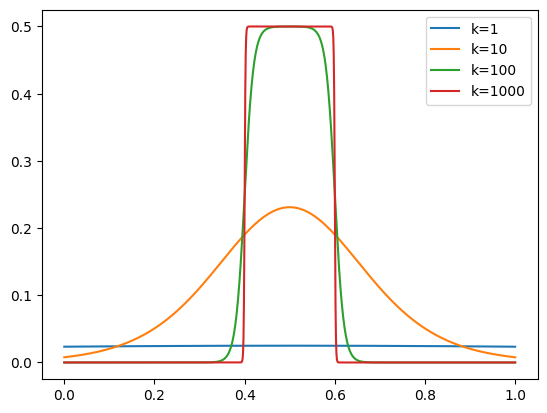
\includegraphics[scale=0.6]{img/bump_functions_1d.png}
      \caption{Bump function approximated with $a = 0.4, b = 0.6$, with differing values of $k$. } 
      \label{fig:bump_functions_1d}
    \end{figure}
  \end{example}

  \begin{example}[Bump Functions in $\mathbb{R}^2$]
    To do this for a 2-D step function, of the form 
    \begin{equation}
      f(x_1, x_2) = \begin{cases} 1 \text{ if } a < x_1 < b \\ 0 & \text{ if else} \end{cases}
    \end{equation}
    this is a simple extension of the first one. We just don't need to make our linear combination dependent on $x_2$ and we're done.
    \begin{equation}
      f(x) \approx \frac{1}{2} \sigma \big( k( x_1 - a)\big) - \frac{1}{2} \sigma \big( k (x_1 - b) \big)
    \end{equation}
  \end{example} 

  \begin{example}[Tower Functions in $\mathbb{R}^2$] 
    Now to construct a tower function of the form 
    \begin{equation}
      f(x_1, x_2) = \begin{cases} 1 & \text{ if } a_1 < x_1 < b_1, a_2 < x_2 < b_2 \\ 0 & \text{ if else} \end{cases}
    \end{equation}
    we need slightly more creativity. Now we can approximate it by doing 
    \begin{equation}
      f(x) \approx \sigma \bigg( k_2 \big[ \sigma\big( k_1 (x_1 - a_1)\big) - \sigma\big( k_1 (x_1 -b_1)\big) + \sigma \big( k_1 (x_2 - a_2)\big) - \sigma\big(k_1 (x_2 - b_2)\big)  big] - b_2\bigg)
    \end{equation}
  \end{example} 

  At this point, we can see how this would extend to $\mathbb{R}^n$, and by isolating parts of the network we can have it approximate tower functions that are completely separate from each other, at any height, and then finally take a linear combination of them to approximate the original function of interest.  

  \begin{theorem}[CS671 Fall 2023 PS5]
    Suppose you have a 2D, $L$-lipschitz function $f(x_1, x_2)$ defined on a unit square ($x_1, x_2 \in \left [0,1 \right ]$). You want to approximate this with an arbitrary neural net $\Tilde{f}$ such that
    \begin{equation}
      \sup_{x \in [0, 1]^2} |f(x) - \Tilde{f}(x)| \leq \epsilon
    \end{equation}
    If we divide the square into a checkerboard of $K \times K$ nonoverlapping squares, approximate the restriction of $f$ to each subsquare with a tower function, what is the least $K$ we would need to ensure that the error is less than $\epsilon$? 
  \end{theorem} 

  Early in the development of the theory of neural nets, An Mei Chen, (currently VP of engineering in Qualcomm) showed in \cite{symmetry} that for certain neural networks, there are multiple parameters $\theta$ that map to the same function $f$. 

  \begin{theorem}[Parameter Symmetry]
    Consider a 2-layer feedforward network of form 
    \begin{equation}
      f = W^{[2]} \circ \sigma \circ W^{[1]}
    \end{equation} 
    where $\sigma = \tanh$. Let $z$ be the hidden vector. We can see that by changing the signs of the $i$th row of $W^{[1]}$, $z_i$'s sign will be flipped. From the properties that $\tanh$ is an odd function (i.e. $\tanh(-x) = - \tanh(x)$), therefore the activation will be also sign-flipped, but this effect can be negated by flipping the $i$th column of the $W^{[2]}$. Therefore, given that $z \in R^{N}$, i.e there are $N$ hidden units, we can choose any set of row-column pairs of the weight matrices to invert, leading to a total of $2^N$ different weightings that produce the same function $f$. 

    Similarly, imagine that we permute the columns of $W^{[2]}$ and rows of $W^{[1]}$ in the same way. Then this will also lead to an invariance in $f$, and so this leads to $N! 2^N$ different weight vectors that lead to the same function! 
  \end{theorem}

\subsection{Tensors} 

  In numerical computing packages like \texttt{numpy} in Python and \texttt{eigen} in C++, we often work with scalars, vectors, and matrices. From linear algebra, the generalization of these objects is a tensor, which is an element of a tensor product space.\footnote{For a refresher, look at my linear algebra notes.} The full mathematical abstraction is rarely needed in practice, and so developers call tensors by their realization as \textit{multidimensional arrays}. 
  
  \begin{definition}[Tensor]
    A \textbf{tensor} is an element of a tensor product space $\bigotimes_i V_i$. It is represented as a \textbf{multidimensional array} of shape $(\dim(V_1), \ldots, \dim(V_n))$. 
  \end{definition}

  If we were trying to build a \texttt{Tensor} class from scratch, what attributes should it have? Well obviously we need the actual data in the tensor, which we will call \texttt{storage}, plus some metadata about the \texttt{shape} (in math, known as the tensor \textit{rank}). Usually, these packages optimize as much as possible for efficiency, and so these are implemented as C-style arrays, which then requires knowledge of the type of each element of the Tensor, called the \texttt{dtype}. Great, with these three attributes, we can do almost every type of arithmetic manipulation. Let's first introduce the most basic math tensor operations, which includes the normal operations supported in an algebra, plus some other ones. We will denote the shapes as well. 
  \begin{enumerate}
    \item \textit{Tensor Addition}. 
    \item \textit{Tensor Additive Inverse}. 
    \item \textit{Scalar Multiplication}. 
    \item \textit{Matrix Multiplication}. 
    \item \textit{Elementwise Multiplication}. 
    \item \textit{Elementwise Multiplicative Inverse}.  
    \item \textit{Transpose}. 
  \end{enumerate} 

  We would probably like some constructors that allows you to directly initialize tensors filled with $0$s (\texttt{zeros}), $1$s (\texttt{ones}), a multiplicative identity (\texttt{eye}\footnote{homophone for $I$, used to denoted the identity matrix.}) Some random initializers would be good, such as sampling from uniforms (\texttt{uniform}), \texttt{gaussians} (\texttt{gaussian}, \texttt{randn}). 

  Finally, we would like some very fundamental operations, such as typecasting, comparison, and indexing as well. 

  \begin{algorithm}[H]
    \caption{Tensor Class Implementation}
    \begin{algorithmic}[1]
    \State \textbf{class} Tensor:
        \State \textbf{Attributes:}
        \State \hspace{1em}storage: array  \Comment{Underlying data storage}
        \State \hspace{1em}shape: tuple    \Comment{Dimensions of tensor}
        \State \hspace{1em}dtype: type     \Comment{Data type of elements}

        \State \textbf{Constructors:}
        \State \texttt{def \_\_init\_\_(data, shape, dtype):}
            \State \hspace{2em}Initialize tensor with given data, shape, and dtype

        \State \textbf{Static Constructors:}
        \State \texttt{@staticmethod}
        \State \texttt{def zeros(shape, dtype):}
            \State \hspace{2em}\Return tensor filled with zeros
        \State \texttt{@staticmethod}
        \State \texttt{def ones(shape, dtype):}
            \State \hspace{2em}\Return tensor filled with ones
        \State \texttt{@staticmethod}
        \State \texttt{def eye(n, dtype):}
            \State \hspace{2em}\Return n×n identity matrix
        \State \texttt{@staticmethod}
        \State \texttt{def uniform(shape, low, high, dtype):}
            \State \hspace{2em}\Return tensor with uniform random values
        \State \texttt{@staticmethod}
        \State \texttt{def gaussian(shape, mean, std, dtype):}
            \State \hspace{2em}\Return tensor with gaussian random values

        \State \textbf{Arithmetic Operations:}
        \State \texttt{def \_\_add\_\_(self, other):}
            \State \hspace{2em}\Return element-wise addition
        \State \texttt{def \_\_neg\_\_(self):}
            \State \hspace{2em}\Return additive inverse
        \State \texttt{def \_\_mul\_\_(self, other):}
            \State \hspace{2em}\Return scalar or element-wise multiplication
        \State \texttt{def matmul(self, other):}
            \State \hspace{2em}\Return matrix multiplication
        \State \texttt{def \_\_truediv\_\_(self, other):}
            \State \hspace{2em}\Return element-wise division
        \State \texttt{def transpose(self):}
            \State \hspace{2em}\Return transposed tensor

        \State \textbf{Utility Operations:}
        \State \texttt{def \_\_repr\_\_(self):}
            \State \hspace{2em}\Return string representation
        \State \texttt{def \_\_str\_\_(self):}
            \State \hspace{2em}\Return human-readable string
        \State \texttt{def \_\_getitem\_\_(self, index):}
            \State \hspace{2em}\Return indexed value(s)
        \State \texttt{def \_\_eq\_\_(self, other):}
            \State \hspace{2em}\Return element-wise equality comparison
    \end{algorithmic}
  \end{algorithm}

  Note that there are other operations, such as concatenation, splitting, and stacking that would be a good idea to implement.  

  \subsubsection{Strides} 

    A specific property of PyTorch is that they use strides as another source of metadata in storing tensors, which greatly speeds up operations. Consider that we want to transpose the first two dimensions of a tensor. Then, we would have to create a new tensor and fill it in with all the elements, which may be too computationally expensive for such a small operation. 

    \begin{definition}[Stride] 
      Given a tensor $T$ of size $(N_1, \ldots N_M)$, it is stored as a contiguous array of $\prod_m T_m$ elements, and we can index it as 
      \begin{equation}
        T[n_1, n_2, \ldots, n_M], \;\;\; 1 \leq n_i \leq N_i
      \end{equation} 
      To counteract this, the \textbf{stride} is a array $S$ of $M$ elements, 
      \begin{equation}
        S = (S_1, \ldots, S_M)
      \end{equation} 
      where indexing with some $I = (n_1, \ldots, n_M)$ is equivalent to computing $S \cdot I$ and taking that index in the array in memory. It defines a mapping. 
    \end{definition}

    If we do some calculation, the default stride of such a vector is defined 
    \begin{equation}
      S_m = \prod_{m < j} N_j, \;\;\; S_M = 1
    \end{equation}

    \begin{example}[Transposing]
      If we want to transpose the tensor above, then we change the stride from 
      \begin{equation}
        S = \bigg( \prod_{1 < j} N_j , \prod_{2 < j} N_j, \ldots, 1 \bigg)
      \end{equation} 
      to 
      \begin{equation}
        S = \bigg( \prod_{2 < j} N_j , \prod_{1 < j} N_j, \ldots, 1 \bigg)
      \end{equation} 
    \end{example}

  \subsubsection{Automatic Differentiation} 

    \begin{lemma}[Derivative of $+/-$]
      Given two tensors $X, Y$ and $Z_+ = X + Y, Z_{-} = X - Y$, we have 
      \begin{align}
        \frac{\partial Z_+}{\partial X} = +1 && \frac{\partial Z_+}{\partial Y} = +1 \\ 
        \frac{\partial Z_-}{\partial X} = +1 && \frac{\partial Z_-}{\partial Y} = -1 
      \end{align}
      where $\pm1$ are tensors of $1$ or $-1$s of the same shape as $X, Y$. 
    \end{lemma}

    \begin{lemma}[Derivative of Element-wise Multiplication]
      Given two tensors $X, Y$ and $Z = X \odot Y$, we have 
      \begin{align}
        \frac{\partial Z}{\partial X} = Y && \frac{\partial Z}{\partial Y} = X
      \end{align}
    \end{lemma} 

    \begin{lemma}[Derivative of Matrix Multiplication]
      Given $X \in (N, M)$ and $Y \in (M, P)$, with $Z = XY \in (N, P)$, the derivative of matrix multiplication is 
      \begin{align}
        \frac{\partial Z}{\partial X} \in (N, P, N, M) && \bigg( \frac{\partial Z}{\partial X} \bigg)_{i, j, k, l} \coloneqq \frac{\partial Z_{i, j}}{\partial X_{k, l}} \\
        \frac{\partial Z}{\partial Y} \in (N, P, M, P) && \bigg( \frac{\partial Z}{\partial Y} \bigg)_{i, j, k, l} \coloneqq \frac{\partial Z_{i, j}}{\partial Y_{k, l}} 
      \end{align} 
    \end{lemma} 

\subsection{Forward and Back Propagation}

  Back in the supervised learning notes, we have gone through the derivation for linear, logistic, and softmax regression. It turns out that despite them having very different architectures, with a identity, sigmoid, and softmax activation function, our choice of loss to be the mean squared loss, the binary cross-entropy, and the cross-entropy loss, had given very cute formulas in computing the gradient of the loss. Unfortunately, the formulas do not get cute when we differentiate neural networks, but they do come in a very structured way. To gain intuition, I would recommend to go over the exercises at the end of the chapter labeled ECE 689 Fall 2021 Midterm. If you just use chain rule to do the calculations, you can see that they require us to compute all the intermediate $z^{(i)}$'s and the $a^{(i)}$'s, a process called \textit{forward propagation}, before we compute the gradients. 

  \begin{definition}[Forward Propagation]
    Given an MLP $f$ and an input $x$, the process of sequentially evaluating 
    \begin{equation}
      x = a^{[0]} \mapsto z^{[1]} \mapsto a^{[1]} \mapsto \ldots \mapsto z^{[L]} \mapsto a^{[L]} = f(x)
    \end{equation}
    is called \textbf{forward propagation}. 
  \end{definition} 

  When we want to compute the derivative of $f$. we can see that the intermediate partial derivatives in the chain rule are repeatedly used. That is, if we have layer $0 \leq l \leq L$, then to compute the derivative with respect to the $l$th layer we use the chain rule 
  \begin{equation}
    \frac{\partial f}{\partial z^{[l]}} = \frac{\partial f}{\partial z^{[l+1]}} \cdot \frac{z^{[l+1]}}{z^{[l]}}
  \end{equation}
  which requires us to know the derivative at the $(l+1)$th layer, along with the current values of $z^{[l]}, z^{[l+1]}$ to evaluate the derivatives at the current point. Therefore, we must complete forward propagation first and then compute \textit{backwards} from the result to the input to compute the gradients. 

  \begin{definition}[Backward Propagation]
    Given an MLP $f$ with input $x$ that has been forward propagated, the process of sequentially evaluating 
    \begin{equation}
      \frac{\partial f}{\partial a^{[L]}} \mapsto \frac{\partial f}{\partial z^{[L]}} \mapsto \ldots \mapsto \frac{\partial f}{\partial z^{[L]}}, 
    \end{equation}
    is called \textbf{backward propagation}, or \textbf{backprop}. 
  \end{definition}

  Backpropagation is not hard, but it is cumbersome notation-wise. What we really want to do is just compute a very long vector with all of its partials $\partial E / \partial \boldsymbol{\theta}$. 

  \begin{algo}[Backpropagation]
    To compute $\frac{\partial E_n}{\partial w_{ji}^{[l]}}$, it would be natural to split it up into a portion where $E_n$ is affected by the term before activation $\mathbf{z}^{[l]}$ and how that is affected by $w_{ji}^{[l]}$. The same goes for the bias terms. 
    \begin{equation}
      \frac{\partial E_n}{\partial w_{ji}^{[l]}} = \underbrace{\frac{\partial E_n}{\partial \mathbf{z}^{[l]}}}_{1 \times N^{[l]}} \cdot \underbrace{\frac{\partial \mathbf{z}^{[l]}}{\partial w_{ji}^{[l]}}}_{N^{[l]} \times 1} \text{ and } \frac{\partial E_n}{\partial b_{i}^{[l]}} = \underbrace{\frac{\partial E_n}{\partial \mathbf{z}^{[l]}}}_{1 \times N^{[l]}} \cdot \underbrace{\frac{\partial \mathbf{z}^{[l]}}{\partial b_{i}^{[l]}}}_{N^{[l]} \times 1}
    \end{equation}
    It helps to visualize that we are focusing on 
    \begin{equation}
      \mathbf{h}_{\boldsymbol{\theta}} (\mathbf{x}) = g\big( \ldots \sigma( \underbrace{\mathbf{W}^{[l]} \mathbf{a}^{[l-1]} + \mathbf{b}^{[l]}}_{\mathbf{z}^{[l]}} )  \ldots \big)
    \end{equation}
    We can expand $\mathbf{z}^{[l]}$ to get 
    \begin{equation}
      \mathbf{z}^{[l]} = \begin{pmatrix} w_{11}^{[l]} & \ldots & w_{1 N^{[l-1]}}^{[l]} \\ \vdots & \ddots & \vdots \\ w_{N^{[l]} 1}^{[l]} & \ldots & w_{N^{[l]} N^{[l-1]}}^{[l]} \end{pmatrix} 
      \begin{pmatrix} a^{[l-1]}_1 \\ \vdots \\ a^{[l-1]}_{N^{[l-1]}} \end{pmatrix} + \begin{pmatrix} b_1^{[l]} \\ \vdots \\ b_{N^{[l]}_{[l]}} \end{pmatrix}
    \end{equation}
    $w_{ji}^{[l]}$ will only show up in the $j$th term of $\mathbf{z}^{[l]}$, and so the rest of the terms in $\frac{\partial \mathbf{z}^{[l]}}{\partial w_{ji}^{[l]}}$ will vanish. The same logic applies to $\frac{\partial \mathbf{z}^{[l]}}{\partial b_{i}^{[l]}}$, and so we really just have to compute 
    \begin{equation}
      \frac{\partial E_n}{\partial w_{ji}^{[l]}} = \underbrace{\frac{\partial E_n}{\partial z^{[l]}_j}}_{1 \times 1} \cdot \underbrace{\frac{\partial z^{[l]}_j}{\partial w_{ji}^{[l]}}}_{1 \times 1} = \delta^{[l]}_j \cdot \frac{\partial z^{[l]}_j}{\partial w_{ji}^{[l]}} \text{ and } \frac{\partial E_n}{\partial b_{i}^{[l]}} = \underbrace{\frac{\partial E_n}{\partial z^{[l]}_j}}_{1 \times 1} \cdot \underbrace{\frac{\partial z^{[l]}_j}{\partial b_{i}^{[l]}}}_{1 \times 1} = \delta^{[l]}_j \cdot \frac{\partial z^{[l]}_j}{\partial b_{i}^{[l]}}
    \end{equation}
    where the $\delta_j^{[l]}$ is called the $j$th \textbf{error term} of layer $l$. If we look at the evaluated $j$th row, 
    \begin{equation}
      z_j^{[l]} = w_{j1}^{[l]} a_1^{[l-1]} + \ldots w_{j N^{[l-1]}} a^{[l-1]}_{N^{[l-1]}} + b_j^{[l]}
    \end{equation}
    We can clearly see that $\frac{\partial z^{[l]}_j}{\partial w_{ji}^{[l]}} = a_i^{[l-1]}$ and $\frac{\partial z^{[l]}_j}{\partial b_{i}^{[l]}} = 1$, which means that our derivatives are now reduced to 
    \begin{equation}
      \frac{\partial E_n}{\partial w_{ji}^{[l]}} = \delta_j^{[l]} a_i^{[l-1]}, \;\;\;\;\; \frac{\partial E_n}{\partial b_{i}^{[l]}} = \delta_j^{[l]}
    \end{equation}
    What this means is that we must know the intermediate values $\mathbf{a}^{[l-1]}$ beforehand, which is possible since we would compute them using forward propagation and store them in memory. Now note that the partial derivatives at this point have been calculated without any consideration of a particular error function or activation function. To calculate $\boldsymbol{\delta}^{[L]}$, we can simply use the chain rule to get 
    \begin{equation}
      \delta_j^{[L]} = \frac{\partial E_n}{\partial z_j^{[L]}} = \frac{\partial E_n}{\partial \mathbf{a}^{[L]}} \cdot \frac{\partial \mathbf{a}^{[L]}}{\partial z_j^{[L]}} = \sum_k \frac{\partial E_n}{\partial a_k^{[L]}} \cdot \frac{\partial a_k^{[L]}}{\partial z_j^{[L]}}
    \end{equation}
    which can be rewritten in the matrix notation
    \begin{equation}
      \boldsymbol{\delta}^{[L]} = \bigg( \frac{\partial \mathbf{g}}{\partial \mathbf{z}^{[L]}} \bigg)^T \bigg( \frac{\partial E_n}{\partial \mathbf{a}^{[L]}} \bigg) = \underbrace{\begin{bmatrix} \frac{\partial g_1}{\partial z_1^{[L]}} & \ldots & \frac{\partial g_{N^{[L]}}}{\partial z^{[L]}_1} \\ \vdots & \ddots & \vdots \\ \frac{\partial g_1}{\partial z^{[L]}_{N^{[L]}}} & \ldots & \frac{\partial g_{N^{[L]}}}{\partial z^{[L]}_{N^{[L]}}} \end{bmatrix}}_{N^{[L]} \times N^{[L]}} \begin{bmatrix} \frac{\partial E_n}{\partial a_1^{[L]}} \\ \vdots \\ \frac{\partial E_n}{\partial a_{N^{[L]}}^{[L]}} \end{bmatrix}
    \end{equation}
    Note that as soon as we make a model assumption on the form of the conditional distribution $Y \mid X = x$ (e.g. it is Gaussian), with it being in the exponential family, we immediately get two things: the loss function $E_n$ (e.g. sum of squares loss), and the canonical link function $\mathbf{g}$
    \begin{enumerate}
      \item If we assume that $Y \mid X = x$ is Gaussian in a regression (of scalar output) setting, then our canonical link would be $g(x) = x$, which gives the sum of squares loss function. Note that since the output is a real-valued scalar, $\mathbf{a}^{[L]}$ will be a scalar (i.e. the final layer is one node, $N^{[L]} = 1$). 
      \begin{equation}
        E_n = \frac{1}{2} (y^{(n)} - a^{[L]} )^2
      \end{equation}
      To calculate $\boldsymbol{\delta}^{[L]}$, we can simply use the chain rule to get 
      \begin{equation}
        \delta^{[L]} = \frac{\partial E_n}{\partial z^{[L]}} = \frac{\partial E_n}{\partial a^{[L]}} \cdot \frac{\partial a^{[L]}}{\partial z^{[L]}} = a^{[L]} - y^{(n)}
      \end{equation}

      \item For classification (of $M$ classes), we would use the softmax activation function (with its derivative next to it for convenience) 
      \begin{equation}
        \mathbf{g}(\mathbf{z}) = \mathbf{g} \bigg( \begin{bmatrix} z_1 \\ \vdots \\ z_M \end{bmatrix} \bigg) = \begin{bmatrix} e^{z_1} / \sum_k e^{z_k} \\ \vdots \\ e^{z_M} / \sum_k e^{z_k} \end{bmatrix}, \;\;\; \frac{\partial g_k}{\partial z_j} = \begin{cases} g_j (1 - g_j) & \text{ if } k = j \\ - g_j g_k & \text{ if } k \neq j \end{cases}
      \end{equation}
      which gives the cross entropy error 
      \begin{equation}
        E_n = - \mathbf{y}^{(n)} \cdot \ln \big( \mathbf{h}_{\boldsymbol{\theta}} (\mathbf{x}^{(n)}) \big) = -\sum_i y^{(n)}_i \, \ln(a_i^{[L]})
      \end{equation}
      where the $\mathbf{y}$ has been one-hot encoded into a standard unit vector in $\mathbb{R}^M$. To calculate $\boldsymbol{\delta}^{[L]}$, we can again use the chain rule again 
      \begin{align}
        \delta_j^{[L]} & = \sum_k \frac{\partial E_n}{\partial a_k^{[L]}} \cdot \frac{\partial a_k^{[L]}}{\partial z_j^{[L]}} \\
        & = - \sum_k \frac{y_k^{(n)}}{a_k^{{[L]}}} \cdot \frac{\partial a_k^{[L]}}{\partial z_j^{[L]}} \\
        & = \bigg( - \sum_{k \neq j} \frac{y_k^{(n)}}{a_k^{{[L]}}} \cdot \frac{\partial a_k^{[L]}}{\partial z_j^{[L]}} \bigg) - \frac{y_j^{(n)}}{a_j^{{[L]}}} \cdot \frac{a_j^{[L]}}{\partial z_j^{[L]}} \\ 
        & = \bigg( - \sum_{k \neq j} \frac{y_k^{(n)}}{a_k^{{[L]}}} \cdot - a_k^{[L]} a_j^{[L]} \bigg) - \frac{y_j^{(n)}}{a_j^{{[L]}}} \cdot a_j^{[L]} (1 - a_j^{[L]}) \\ 
        & = a_j^{[L]} \underbrace{\sum_{k} y_k^{(n)}}_{1} - y_j^{(n)} = a_j^{[L]} - y_j^{(n)}
      \end{align}
      giving us 
      \begin{equation}
        \boldsymbol{\delta}^{[L]} = \mathbf{a}_j^{[L]} - \mathbf{y}^{[L]}
      \end{equation}
    \end{enumerate}

    Now that we have found the error for the last layer, we can continue for the hidden layers. We can again expand by chain rule that 
    \begin{equation} 
      \delta_j^{[l]} = \frac{\partial E_n}{\partial z_j^{[l]}} = \frac{\partial E_n}{\partial \mathbf{z}^{[l+1]}} \cdot \frac{\partial \mathbf{z}^{[l+1]}}{\partial z_j^{[l]}} = \sum_{k=1}^{N^{[l+1]}} \frac{\partial E_n}{\partial z_k^{[l+1]}} \cdot \frac{\partial z_k^{[l+1]}}{\partial z_j^{[l]}} = \sum_{k=1}^{N^{[l+1]}} \delta_k^{[l+1]} \cdot \frac{\partial z_k^{[l+1]}}{\partial z_j^{[l]}}
    \end{equation} 
    By going backwards from the last layer, we should already have the values of $\delta_k^{[l+1]}$, and to compute the second partial, we recall the way $a$ was calculated 
    \begin{equation}
      z_k^{[l+1]} = b_k^{[l+1]} + \sum_{j=1}^{N^{[l]}} w_{kj}^{[l+1]} \sigma(z_j^{[l]}) \implies \frac{\partial z_k^{[l+1]}}{\partial z_j^{[l]}} = w_{kj}^{[l+1]} \cdot \sigma^\prime(z_j^{[l]})
    \end{equation}
    Now this is where the ``back" in backpropagation comes from. Plugging this into the equation yields a final equation for the error term in hidden layers, called the \textbf{backpropagation formula}: 
    \begin{equation}
      \delta_j^{[l]} = \sigma^\prime(z_j^{[l]}) \sum_{k=1}^{N^{[l+1]}} \delta_k^{[l+1]} \cdot w_{kj}^{[l+1]}
    \end{equation}
    which gives the matrix form 
    \begin{equation}
      \boldsymbol{\delta}^{[l]} = \boldsymbol{\sigma}^\prime (\mathbf{z}^{[l]}) \odot (\mathbf{W}^{[l+1]})^T \boldsymbol{\delta}^{[l+1]} = \begin{bmatrix} \sigma^\prime (z_1^{[l]}) \\ \vdots \\ \sigma^\prime (z_{N^{[L]}}^{[l]})\end{bmatrix} \odot \begin{bmatrix} w_{11}^{[l+1]} & \ldots & w^{[l+1]}_{N^{[l+1]} 1} \\ \vdots & \ddots & \vdots \\ w^{[l+1]}_{1 N^{[l]}} & \ldots & w^{[l+1]}_{N^{[l+1]} N^{[l]}} \end{bmatrix} \begin{bmatrix} \delta_1^{[l+1]} \\ \vdots \\ \delta_{N^{[l+1]}}^{[l+1]} \end{bmatrix} 
    \end{equation}
    and putting it all together, the partial derivative of the error function $E_n$ with respect to the weight in the hidden layers for $1 \leq l < L$ is 
    \begin{equation}
      \frac{\partial E_n}{\partial w_{ji}^{[l]}} = a_i^{[l-1]} \sigma^\prime(z_j^{[l]}) \sum_{k=1}^{N^{[l+1]}} \delta_k^{[l+1]} \cdot w_{kj}^{[l+1]} 
    \end{equation}
  \end{algo}

  A little fact is that the time complexity of both forward prop and back prop should be the same, so if you ever notice that the time to compute these two functions scales differently, you're probably making some repeated calculations somewhere. 

  \begin{algo}[Epoch of Training]
    Before training, we initialize all the parameters to be 
    \begin{equation}
      \boldsymbol{\theta} = (\mathbf{W}^{[1]}, \mathbf{b}^{[1]}, \mathbf{W}^{[2]}, \ldots, \mathbf{W}^{[L]}, \mathbf{b}^{[L]})
    \end{equation} 
    Then, we repeat the following for one epoch of training. 
    \begin{enumerate}
      \item \textit{Choose Batch}: We choose an arbitrary data point $(\mathbf{x}^{(n)}, \mathbf{y}^{(n)})$, an minibatch, or the entire batch to compute the gradients on. 
      
      \item \textit{Forward Propagation}: Apply input vector $\mathbf{x}^{(n)}$ and use forward propagation to compute the values of all the hidden and activation units 
      \begin{equation}
        \mathbf{a}^{[0]} = \mathbf{x}^{(n)}, \mathbf{z}^{[1]}, \mathbf{a}^{[1]}, \ldots, \mathbf{z}^{[L]}, \mathbf{a}^{[L]} = h_{\boldsymbol{\theta}} (\mathbf{x}^{(n)})
      \end{equation}
      
      \item \textit{Back Propagation}: 
      \begin{enumerate}
        \item Evaluate the $\boldsymbol{\delta}^{[l]}$'s starting from the back with the formula 
        \begin{align}
          \boldsymbol{\delta}^{[L]} & = \bigg( \frac{\partial \mathbf{g}}{\partial \mathbf{z}^{[L]}} \bigg)^T \bigg( \frac{\partial E_n}{\partial \mathbf{a}^{[L]}} \bigg) \\
          \boldsymbol{\delta}^{[l]} & = \boldsymbol{\sigma}^\prime (\mathbf{z}^{[l]}) \odot (\mathbf{W}^{[l+1]})^T \boldsymbol{\delta}^{[l+1]} \;\;\;\;\; l = 1, \ldots, L-1
        \end{align}
        where $\frac{\partial \mathbf{g}}{\partial \mathbf{z}^{[L]}}$ can be found by taking the derivative of the known link function, and the rest of the terms are found by forward propagation (these are all functions which have been fixed in value by inputting $\mathbf{x}^{(n)}$).  

        \item Calculate the derivatives of the error as 
        \begin{equation}
          \frac{\partial E_n}{\partial \mathbf{W}^{[l]}} = \boldsymbol{\delta}^{[l]} (\mathbf{a}^{[l-1]})^T, \;\;\;\;\; \frac{\partial E_n}{\partial \mathbf{b}^{[l]}} = \boldsymbol{\delta}^{[l]}
        \end{equation}
      \end{enumerate}
      
      \item \textit{Gradient Descent}: Subtract the derivatives with step size $\alpha$. That is, for $l = 1, \ldots, L$, 
      \begin{equation}
        \mathbf{W}^{[l]} = \mathbf{W}^{[l]} - \alpha \frac{\partial E_n}{\partial \mathbf{W}^{[l]}} , \;\;\;\;\; \mathbf{b}^{[l]} = \mathbf{b}^{[l]} - \alpha \frac{\partial E_n}{\partial \mathbf{b}^{[l]}}
      \end{equation}
      The specific optimizer can differ, e.g. Adam, SGD, BFGS, etc., but the specific algorithm won't be covered here. It is common to use Adam, since it usually works better. If we can afford to iterate over the entire batch, L-BFGS may also be useful. 
    \end{enumerate}
  \end{algo}

  \begin{code}[Neural Net from Scratch]
    Now it's time to implement what most newcomers fear most: a neural net from scratch using only numpy. Doing this will get you to understand the inner workings of a neural net, and you can find the relevant code \href{code/mlp_from_scratch.ipynb}{here}.  
  \end{code} 

  \begin{code}[Pytorch Implementation of Forward and Backward Propagation]
    Once you have finished implementing from scratch, you can now use the PyTorch API to access the same model weights. The code \href{code/forward_backward.ipynb}{here} shows how to look at the forward propagation and backpropagation steps in PyTorch in intermediate layers and shows the backend behind storing gradients. 
  \end{code}

\subsection{Overparamterization is Good?} 

  Given that the input dimension is $D$, say that all the hidden layers are of dimension $D$ and we have $L$ layers. Then, we are storing a matrix (plus bias vector) at each layer, resulting in a scaling of $O(D^2 L)$. This quadratic scaling leads to overparameterized models, which should raise a red flag. This naturally leads to overfitting, but a strange phenomenon occurs.\footnote{I found this from Lex Fridman's podcast with Ilya Sutskever.}  
  \begin{enumerate}
    \item In the beginning, the training loss goes down along with the validation loss. 
    \item Soon the validation loss starts to go up while the training loss goes down, leading to overfitting. 
    \item The overfitting is worst when the training loss is $0$. 
    \item At this point, the training loss remains at $0$, but generalization starts to improve, and mysteriously the validation loss starts going down. 
  \end{enumerate}

  There are many theories of why the last step ever happens. To interpret this, let's revisit what overfitting means. It means that small perturbations of the inputs will result in large variances in the outputs. If we generalize well, $x + \epsilon$ should also result in $f(x) + O(\epsilon)$. Therefore, this means that the more parameters it has, the better this stability is and therefore the more robust the model. How should we measure this sense of stability? In analysis, a metric to assess the robustness of a deep neural net $f_\theta: \mathbb{R}^n \longrightarrow \mathbb{R}^m$ is its Lipshitz constant, which effectively bounds how much $f$ can change given some change in $x$. 

  \begin{definition}[Lipshitz Continuity]
    A function $f: \mathbb{R}^n \longrightarrow \mathbb{R}^m$ is called \textbf{Lipshitz continuous} if there exists a constant $L$ such that for all $x, y \in \mathbb{R}^n$
    \begin{equation}
      ||f(x) - f(y)||_2 \leq L ||x - y||_2
    \end{equation}
    and the smallest $L$ for which the inequality is true is called the \textbf{Lipshitz constant}, denoted $\mathrm{Lip}(f)$. 
  \end{definition}

  \begin{theorem}[Lipschitz Upper Bound with Operator Norm of Total Derivative]
    If $f: \mathbb{R}^n \longrightarrow \mathbb{R}^m$ is Lipschitz continuous, then 
    \begin{equation}
      \mathrm{Lip}(f) = \sup_{x \in \mathbb{R}^n} ||D_x f||_{\mathrm{op}}
    \end{equation}
    where $||\cdot ||_{\mathrm{op}}$ is the operator norm of a matrix. In particular, if $f$ is scalar-valued, then its Lipschitz constant is the maximum norm of its gradient on its domain 
    \begin{equation}
      \mathrm{Lip}(f) = \sup_{x \in \mathbb{R}^n} ||\nabla f(x)||_2
    \end{equation}
  \end{theorem}

  The above theorem makes sense, since indeed the stability of the function should be equal to the stability of its "maximum" linear approximation $D_x f$. 

  \begin{theorem}[Lipschitz Upper Bound for MLPs]
    It has already been shown that for a $K$-layer MLP
    \begin{equation}
      h_\theta (\mathbf{x}) \coloneqq \mathbf{T}_K \circ \boldsymbol{\rho}_{K-1} \circ \mathbf{T}_{K-1} \circ \cdots \circ \boldsymbol{\rho}_1 \circ \mathbf{T}_1 (\mathbf{x})
    \end{equation}
    the Lipshitz constant for an affine map $\mathbf{T}_k (\mathbf{x}) = M_k \mathbf{x} + b_k$ is simply the operator norm (largest singular value) of $M_k$, while that of an activation function is always bounded by some well-known constant, usually $1$. So, the Lipshitz constant of the entire composition $h$ is simply the product of all operator norms of $M_k$. 
  \end{theorem}

  What about $K$-computable functions in general? That is, given a function $f: \mathbb{R}^n \longrightarrow \mathbb{R}^m$ with 
  \begin{align}
    v_0 (\mathbf{x}) & = \mathbf{x} \\ 
    v_1 (\mathbf{x}) & = g_1 \big(v_0(\mathbf{x}) \big) \\
    v_2 (\mathbf{x}) & = g_2 \big(v_0(\mathbf{x}), v_1 (\mathbf{x}) \big) \\ 
    \ldots & = \ldots \\
    v_k (\mathbf{x}) & = g_k \big(v_0 (\mathbf{x}), v_1(\mathbf{x}), \ldots, v_{k-1} (\mathbf{x}) \big) \\
    \ldots & = \ldots \\
    v_K (\mathbf{x}) & = g_K \big(v_0(\mathbf{x}), v_1 (\mathbf{x}), \ldots, v_{K-2}(\mathbf{x}), v_{K-1}(\mathbf{x}) \big)
  \end{align}
  where $v_k: \mathbb{R}^n \longrightarrow \mathbb{R}^{n_k}$, with $n_0 = n$ and $n_K = m$, and 
  \begin{equation}
    g_k : \prod_{i=0}^{k-1} \mathbb{R}^{n_i} \longrightarrow \mathbb{R}^{n_k}
  \end{equation}
  To differentiate $v_k$ w.r.t. $\mathbf{x}$, we can use the chain rule, resulting in the total derivative 
  \begin{equation}
    \underbrace{\frac{\partial v_k}{\partial \mathbf{x}}}_{n_k \times n} = \sum_{i=1}^{k-1} \underbrace{\frac{\partial g_k}{\partial v_i}}_{n_k \times n_i} \, \underbrace{\frac{\partial v_i}{\partial \mathbf{x}}}_{n_i \times n}
  \end{equation}

  Therefore, it is this Lipschitz property that might entail how stable an MLP is. We have seen from the universal approximation theorems that for a data set of any size, we can always fit a one-layer perceptron that perfectly fits through all of them, given that the layer is large enough. In these cases, we are interested in fitting the data \textit{smoothly}, and theoretical research in bounding the Lipschitz constant is popular.

  In practice this behavior is reflected in \textit{most} cases, but they may be very sensitive in some cases, which we call \textit{adversarial examples}. Adversarial examples take advantage of this weakness by adding carefully chosen perturbations that drastically change the output of the network. Adversarial machine learning attempts to study these weaknesses and hopefully use them to create more robust models. It is natural to expect that the precise configuration of the minimal necessary perturbations is a random artifact of the normal variability that arises in different runs of backpropagation learning. Yet, it has been found that adversarial examples are relatively robust, and are shared by neural networks with varied number of layers, activations or trained on different subsets of the training data. This suggest that the deep neural networks that are learned by backpropagation have \textit{intrinsic} blind spots, whose structure is connected to the data distribution in a non-obvious way. 

\subsection{Engineering Heuristics}

  \subsubsection{Weight Initialization}

    The way that we initialize our weights can have a huge impact on our training performance. Imagine that you are creating the first neural network and you want to decide how to initialize it. You may consider many different cases. 

    \begin{example}[Constant Initialization]
      You may first think of initializing everything to $0$ or $1$, which is the simplest. Let's run this, but we can already see by epoch 15 that we have some problems. 
      \begin{center}
        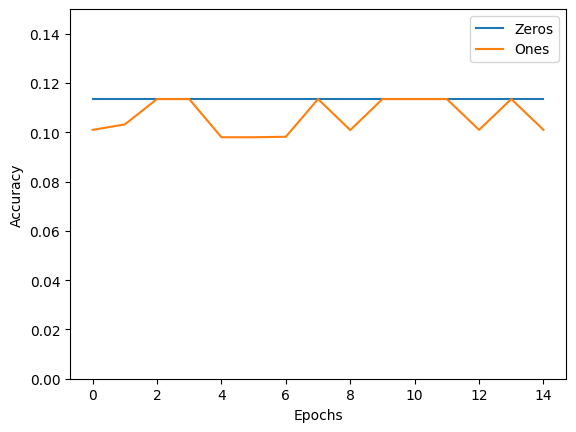
\includegraphics[scale=0.5]{img/first_initialize.png}
      \end{center}
      Clearly, this is not good, and theoretically this makes sense since it means all our activations are going to be the same, and thus all our gradients will be the same, meaning that are updates will be the same for every weight, which is not good mixing. We can see this below: 
    \end{example}

    \begin{example}[Random Initialization with High Variance]
      Okay, this didn't work, so perhaps you think it would be a good idea have more randomness to the initialization so that all the weights aren't exactly one number. You could think of initializing everything with three distinct schemes: 
      \begin{enumerate}[itemsep=0mm] 
        \item Randomly initialize everything to be $-1$ or $1$ with equal probability. 
        \item Randomly initialize everything to be a Gaussian random variable with standard deviation $1$. 
        \item Randomly initialize everything to be a uniform random variable between $-1$ and $1$. 
      \end{enumerate}
      Running the experiments give the following. 
      \begin{center} 
        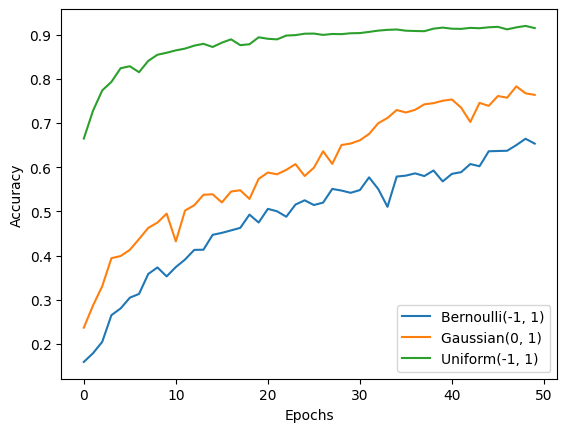
\includegraphics[scale=0.5]{img/second_initialization.png}
      \end{center}
      However, this is also not good since it means that the activations will be very large, and thus the gradients will be very large, and so the updates will be very large. This is not good since it means that the weights will be jumping around a lot, and we won't be able to converge. Furthermore, depending on what activations we choose, e.g. tanh or sigmoid, very large activations may saturate the gradients and kill the learning. 
    \end{example}

    \begin{example}[Random Initialization with Low Variance]
      This improves the next problem but now you want to fix the situation of the gradients being too big. Therefore, you should initialize the parameters to be smaller values, but not so small that they are zeros and we have the same problem as before. We use improved schemes: 
      \begin{enumerate}[itemsep=0mm] 
        \item Randomly initialize everything to be $-0.1$ or $0.1$ with equal probability. 
        \item Randomly initialize everything to be a Gaussian random variable with standard deviation $0.1$. 
        \item Randomly initialize everything to be a uniform random variable between $-0.1$ and $0.1$.
      \end{enumerate}
      \begin{center}
        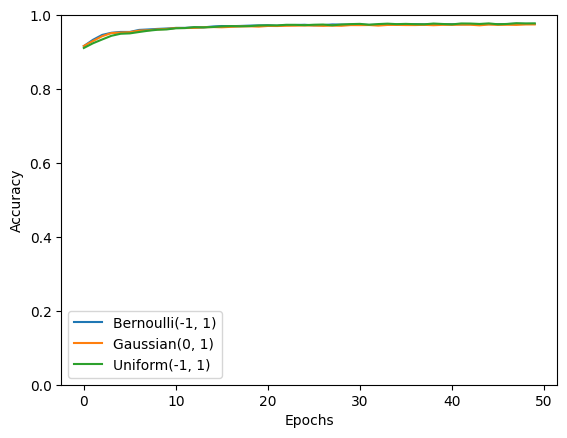
\includegraphics[scale=0.5]{img/third_initialize.png}
      \end{center}
    \end{example}

    Through out experiments, we have learned that a good rule of thumb for initializing weights is to make them small and uniformly random without being too small. While it is harder to get better than this for MNIST, a slightly better approach is Xavier initialization, which builds upon our same ideas. 

    \begin{definition}[Xavier Initialization]
      The \textbf{Xavier initialization} simply initializes each weight as a uniform distribution, with its range dependent on the size of the input. 
      \begin{equation}
        w_{ij}^{[l]} \sim U \bigg( -\frac{1}{\sqrt{N^{[l-1]}}}, \frac{1}{\sqrt{N^{[l-1]}}} \bigg)
      \end{equation}
      where $N^{[l-1]}$ is the number of neurons in the previous layer. This is a good rule of thumb for the weights, but the biases can be initialized to $0$ (though they are also initialized uniformly by default).
    \end{definition}

    \begin{code}[Experimenting with Weight Initializations] 
      The code used for generating the figures can be found \href{code/initialization.ipynb}{here}. 
    \end{code}
    
  \subsubsection{Activation Functions} 

    The choice of the activation function can have a significant impact on your training, and we will describe a few examples below. The first thing to note is that we must ensure that there is a nonzero gradient almost everywhere. If, for example, we had a piecewise constant activation function, the gradient is $0$ almost everywhere, and it would kill the gradient of the entire network. In the early days of deep learning, researchers used the probability-inspired sigmoid and tanh functions as the main source of nonlinearity. Let's go over them below. 

    \begin{definition}[Sigmoid]
      Sigmoid activations are historically popular since they have a nice interpretation as a saturating ``fire rate" of a neuron. However, there are 3 problems: 
      \begin{enumerate}
        \item The saturated neurons ``kill" the gradients, since if the input at any one point in the layers is too positive or negative, the gradient will vanish, making very small updates. This is known as the \textbf{vanishing gradient problem}. Therefore, the more layers a neural network has, the more likely we are to see this vanishing gradient problem. 
        \item Sigmoid functions are not zero centered (i.e. its graph doesn't cross the point $(0, 0)$ ). Consider what happens when the input $x$ to a neuron is always positive. Then, the sigmoid $f$ will have a gradient of 
        \begin{equation}
          f \bigg( \sum_i w_i x_i + b \bigg) \implies \frac{\partial f}{\partial w_i} = f^\prime \bigg( \sum_i w_i x_i + b \bigg)\, x_i
        \end{equation}
        which means that the gradients $\nabla_\mathbf{w} f$ will always have all positive elements or all negative elements, meaning that we will be restricted to moving in certain nonoptimal directions when updating our parameters. 
      \end{enumerate}
    \end{definition} 

    \begin{definition}[Hyperbolic Tangent]
      The hyperbolic tangent is zero centered, which is nice, but it still squashes numbers to range $[-1, 1]$ and therefore kills the gradients when saturated. 
    \end{definition}

    It turns out that these two activations were ineffective in deep learning due to saturation. A less probability inspired activation was the ReLU, which showed better generalization an speed of convergence. 

    \begin{definition}[Rectified Linear Unit]
      The ReLU function has the following properties: 
      \begin{enumerate}
          \item It does not saturate in the positive region. 
          \item It is very computationally efficient (and the fact that it is nondifferentiable at one point doesn't really affect computations). 
          \item It converges much faster than sigmoid/tanh in practice. 
          \item However, note that if the input is less than $0$, then the gradient of the ReLU is $0$. Therefore, if we input a vector that happens to have all negative values, then the gradient would vanish and we wouldn't make any updates. These ReLU ``dead zones" can be a problem since it will never activate and never update, which can happen if we have bad initialization. A more common case is when your learning rate is too high, and the weights will jump off the data manifold. 
      \end{enumerate}
    \end{definition}

    Unfortunately, the ReLU had some weaknesses, mainly being the \textit{dying ReLU}, which is when the ReLU is stuck in the negative region and never activates. This is a problem since the gradient is $0$ in the negative region, and so the weights will never update. Therefore, some researchers have proposed some modifications to the ReLU. 

    \begin{definition}[Leaky ReLU]
      The leaky ReLU 
      \begin{equation}
        \sigma(x) = \max\{0.01 x, x\}
      \end{equation}
      does not saturate (i.e. gradient will not die), is computationally efficient, and converges much faster than sigmoid/tanh in practice. We can also parameterize it with $\alpha$ and have the neural net optimize $\alpha$ along with the weights. 
      \begin{equation}
        \sigma(x) = \max\{\alpha x, x\}
      \end{equation}
    \end{definition}

    \begin{definition}[ELU]
      The exponential linear unit has all the benefits of ReLU, with closer to mean outputs. It has a negative saturation regime compared with leaky ReLU, but it adds some robustness to noise. 
      \begin{equation}
        \sigma(x) = \begin{cases} x & \text{ if } x > 0 \\ \alpha \big(\exp{x} - 1 \big) & \text{ if } x \leq 0 \end{cases}
      \end{equation}
    \end{definition}

    \begin{definition}[SELU]
      The scaled exponential linear unit is a self-normalizing activation function, which means that it preserves the mean and variance of the input. This is useful for deep networks, since the mean and variance of the input will be preserved through the layers. Its formula is 
      \begin{equation}
        \sigma(x) = \lambda \begin{cases} x & \text{ if } x > 0 \\ \alpha \big(\exp{x} - 1 \big) & \text{ if } x \leq 0 \end{cases}
      \end{equation}
      where $\lambda$ and $\alpha$ are constants.
    \end{definition}
    
    Later on, some further modifications were made, such as the \textbf{Swish} and the \textbf{Mish} \cite{mish} activation functions. These functions have a distinctive negative concavity, unlike ReLU, which accounts for preservation of small negative weights.  

    \begin{definition}[Swish]
      The Swish activation function is defined as 
      \begin{equation}
        \sigma(x) = x \cdot \sigma(\beta x) 
      \end{equation}
      where $\beta$ is a parameter that can be learned. 
    \end{definition}

    \begin{definition}[Mish]
      The Mish activation function is defined as 
      \begin{equation}
        \sigma(x) = x \cdot \tanh(\ln(1 + \exp(x))) 
      \end{equation}
    \end{definition}

    \begin{code}[Generating Graphs] 
      Code used to generate these graphs are \href{code/activation_functions.ipynb}{here}.
    \end{code} 

  \subsection{Datasets and Dataloaders} 

    For here, we will go over some of the main datasets that are used in deep learning. 

    \begin{definition}[MNIST and Fashion MNIST]
      The MNIST dataset consists of 60k training images and 10k test images of handwritten digits. The Fashion MNIST dataset consists of 60k training images and 10k test images of clothing items. These are considered quite easy with the basic benchmarks: 
      \begin{enumerate} 
        \item Linear classifiers can reach past 90\% accuracy. 
        \item A 2 layer MLP can reach up to 97\% accuracy. 
        \item A CNN can reach up to 99\% accuracy. 
      \end{enumerate}
    \end{definition}

    \begin{definition}[CIFAR10 and CIFAR 100]
      The CIFAR10 dataset consists of 60k 32x32 color images in 10 classes, with 6k images per class. The CIFAR100 dataset consists of 60k 32x32 color images in 100 classes, with 600 images per class. These are considered quite hard with the basic benchmarks: 
      \begin{enumerate} 
        \item Linear classifiers can reach past 40\% accuracy. 
        \item A 2 layer MLP can reach up to 60\% accuracy. 
        \item A CNN can reach up to 80\% accuracy. 
      \end{enumerate}
    \end{definition}

    \begin{definition}[ImageNet]
      The ImageNet dataset, created at Stanford by Fei-Fei Li \cite{ImageNet}, consists of 1.2 million training images and 50k validation images in 1000 classes. This is considered very hard with the basic benchmarks. 
    \end{definition}

    Creating your own custom dataset with spreadsheets or images is easy.\footnote{https://pytorch.org/tutorials/beginner/data\_loading\_tutorial.html} Loading it to a dataloader that shuffles and outputs minibatches of data is trivial. However, when doing so, you should pay attention to a couple things. 
    \begin{enumerate} 
      \item Batch size: The dataloader stores the dataset (which can be several hundred GBs) in the drive, and extracts batches into memory for processing. You should set your batch sizes so that they can fit into the GPU memory, which is often smaller than the CPU memory. 
    \end{enumerate}

\subsection{Exercises} 

  \begin{exercise}[Tarokh, ECE685 2021 Midterm 1.1]
    Let $x \in \mathbb{R}$ denote a random variable with the following \textit{cumulative distribution function} 
    \begin{equation}
      F(x) = \exp \bigg( - \exp \bigg( - \frac{x - \mu}{\beta} \bigg) \bigg)
    \end{equation}
    where $\mu$ and $\beta > 0$ denote the location and scale parameters, respectively. Let $\mathcal{D} = \{x_1, \ldots, x_n\}$ be a set of $n$ iid observations of $x$. 
    \begin{enumerate}
      \item Write an equation for a cost function $L(\mu, \beta \mid \mathcal{D})$ whose minimization gives the maximum likelihood estimates for $\mu$ and $\beta$. 
      \item Compute the derivatives of $L(\mu, \beta \mid \mathcal{D})$ with respect to $\mu$ and $\beta$ and write a system of equations whose solution gives the MLEs of $\mu$ and $\beta$. 
    \end{enumerate}
  \end{exercise}
  \begin{solution}
    We can derive the PDF of the observation as 
    \begin{equation}
      f(x; \mu, \beta) = \frac{d F(x)}{dx} = \frac{1}{\beta} \exp \bigg\{ - \bigg( \frac{x - \mu}{\beta} + \exp \Big( - \frac{x - \mu}{\beta}\Big) \bigg) \bigg\}
    \end{equation}
    and the likelihood is then 
    \begin{equation}
      L(\mu, \beta \mid \mathcal{D}) = \prod_{i=1}^N \frac{1}{\beta} \exp \bigg\{ - \bigg( \frac{x^{(i)} - \mu}{\beta} + \exp \Big( - \frac{x^{(i)} - \mu}{\beta}\Big) \bigg) \bigg\}
    \end{equation}
    Rather than maximizing this likelihood, we minimize the negative log of it, defined as 
    \begin{equation}
      \ell(\mu, \beta \mid \mathcal{D}) = - \ln L(\mu, \beta \mid \mathcal{D}) = N \ln{\beta} + \frac{\sum_{i} x^{(I)} - N \mu}{\beta} + \sum_{i=1}^N \exp \Big( - \frac{x^{(i)} - \mu}{\beta} \Big)
    \end{equation}
    The derivatives of $\ell$ can be computed simply by using the derivative rules.  
    \begin{align}
      \frac{\partial \ell}{\partial \mu} & = - \frac{N}{\beta} + \frac{1}{\beta} \sum_{i=1}^N \exp \Big( - \frac{x^{(i)} - \mu}{\beta} \Big) \\
      \frac{\partial \ell}{\partial \beta} & = \frac{N}{\beta} - \frac{\sum_{i} x^{(i)} - N \mu}{\beta^2} + \frac{1}{\beta^2} \sum_{i=1}^N (x^{(i)} - \mu) \exp \Big( - \frac{x^{(i)} - \mu}{\beta} \Big)
    \end{align}
    and so the MLE estimates that minimizes $\ell$ can be found by setting the equations above equal to $0$. 
  \end{solution}

  \begin{exercise}[ECE 685 Fall 2021 Midterm 1.2]
    The figure depicts a simple neural network with one hidden layer. The inputs to the network are denoted by $x_1, x_2, x_3$, and the output is denoted by $y$. The activation functions of the neurons in the hidden layer are given by $h_1 (z) = \sigma(z), h_2 (z) = \tanh(z)$, and the output unit activation function is $g(z) = z$, where $\sigma(z) = \frac{1}{1 + \exp(-z)}$ and $\tanh(z) = \frac{\exp(z) - \exp(-z)}{\exp(z) + \exp(-z)}$ are the logistic sigmoid and hyperbolic tangent, respectively. The biases $b_1, b_2$ are added to the inputs of the neurons int he hidden layer before passing them through the activation functions. let 
    \begin{equation}
      \mathbf{w} = (b_1, b_2, w_{11}^{(1)}, w_{12}^{(1)}, w_{21}^{(1)}, w_{31}^{(1)}, w_{32}^{(1)}, w_1^{(2)}, w_2^{(2)})
    \end{equation}
    denote the vector of network parameters. 
    \begin{enumerate}
      \item Write the input output relation $y = f(x_1, x_2, x_3 ; \mathbf{w})$ in explicit form. 

      \item Let $\mathcal{D} = \{(x_{1, n}, x_{2, n}, x_{3, n})\}$ denote a training dataset of $N$ points where $y_n \in \mathbb{R}$ are labels of the corresponding data points. We want to estimate the network parameters $\mathbf{w}$ using $\mathcal{D}$ by minimizing the mean squared error loss 
      \begin{equation}
        L(\mathbf{w}) = \frac{1}{2} \sum_{n=1}^N \big( f(x_{1, n}, x_{2, n}, x_{3, n}; \mathbf{w}) - y_n \big)^2
      \end{equation}
      Compute the gradient of $L(\mathbf{w})$ with respect to the network parameters $\mathbf{w}$. 

      \item Write pseudo code for one iteration for minimizing $L(\mathbf{w})$ with respect to the network parameters $\mathbf{w}$ using SGD with learning rate $\eta > 0$. 
    \end{enumerate}

    \begin{center}
      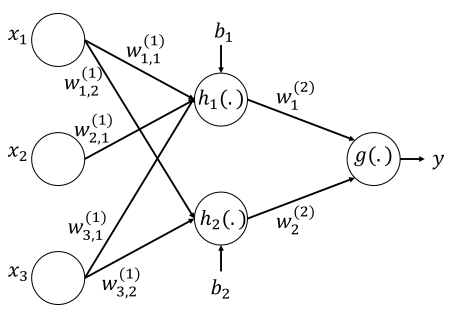
\includegraphics[scale=0.4]{img/tarokhfig1.png}
    \end{center}
  \end{exercise}
  \begin{solution}
    We can write the computation graph as 
    \begin{align} 
      z_1^{(1)} & = w_{11}^{(1)} x_1 + w_{21}^{(1)} x_2 + w_{31}^{(1)} x_3 + b_1 \\
      z_2^{(1)} & = w_{12}^{(1)} x_1 + w_{32}^{(1)} x_3 + b_2 \\
      a_1^{(1)} & = \sigma(z^{(1)})\\
      a_2^{(1)} & = \tanh(z_2^{(1)}) \\
      z^{(2)} & = w_{1}^{(2)} a_1^{(1)} + w_2^{(2)} a_2^{(1)} \\
      y = a^{(2)} & = g(z^{(2)})
    \end{align}
    and composing these gives 
    \begin{equation}
      y = w_1^{(2)} \sigma(w_{11}^{(1)} x_1  + w_{21}^{(1)} x_2 + w_{31}^{(1)} x_3 + b_1) + w_2^{(2)} \tanh(w_{12}^{(1)} x_1 + w_{32}^{(1)} x_3 + b_2)
    \end{equation}
    The gradient of the network can be written as 
    \begin{align}
      \nabla_\mathbf{w} L(\mathbf{w}) & = \frac{1}{2} \sum_{n=1}^N \nabla_\mathbf{w} \big( f(x_{1, n}, x_{2, n}, x_{3, n}; \mathbf{w}) - y_n \big)^2 \\
      & = \sum_{n=1}^N (f(x_{1, n}, x_{2, n}, x_{3, n}; \mathbf{w}) - y_n) \nabla_\mathbf{w} f(x_{1, n}, x_{2, n}, x_{3, n})
    \end{align}
    where 
    \begin{equation}
      \nabla_\mathbf{w} f(x_{1, n}, x_{2, n}, x_{3, n}) = \frac{\partial f}{\partial \mathbf{w}} \bigg|_{\mathbf{x} = \mathbf{x}^{(n)}}
    \end{equation}
    Now we can take derivatives using chain rule, working backwards, and using the derivative identities $\sigma^\prime (z)  = \sigma(z) (1 - \sigma(z))$ and $\tanh^\prime (z) = 1 - \tanh^2 (z)$. 
    \begin{align}
        \frac{\partial f}{\partial w_1^{(2)}} & = \frac{\partial f}{\partial z^{(2)}} \frac{\partial z^{(2)}}{\partial w_1^{(2)}} = a_1^{(1)} \\
        \frac{\partial f}{\partial w_2^{(2)}} & = \frac{\partial f}{\partial z^{(2)}} \frac{\partial z^{(2)}}{\partial w_2^{(2)}} = a_2^{(1)} \\ 
        \frac{\partial f}{\partial w_{11}^{(1)}} & = \frac{\partial f}{\partial z^{(2)}} \frac{\partial z^{(2)}}{\partial a^{(1)}_1} \frac{\partial a^{(1)}_1}{\partial z_1^{(1)}} \frac{\partial z_1^{(1)}}{\partial w_{11}^{(1)}} = w_1^{(2)} a_1^{(1)} (1 - a_1^{(1)}) x_1\\
        \frac{\partial f}{\partial w_{21}^{(1)}} & = \frac{\partial f}{\partial z^{(2)}} \frac{\partial z^{(2)}}{\partial a^{(1)}_1} \frac{\partial a^{(1)}_1}{\partial z_1^{(1)}} \frac{\partial z_1^{(1)}}{\partial w_{21}^{(1)}} = w_1^{(2)} a_1^{(1)} (1 - a_1^{(1)}) x_2\\
        \frac{\partial f}{\partial w_{31}^{(1)}} & = \frac{\partial f}{\partial z^{(2)}} \frac{\partial z^{(2)}}{\partial a^{(1)}_1} \frac{\partial a^{(1)}_1}{\partial z_1^{(1)}} \frac{\partial z_1^{(1)}}{\partial w_{31}^{(1)}} = w_1^{(2)} a_1^{(1)} (1 - a_1^{(1)}) x_3\\
        \frac{\partial f}{\partial b_{1}} & = \frac{\partial f}{\partial z^{(2)}} \frac{\partial z^{(2)}}{\partial a^{(1)}_1} \frac{\partial a^{(1)}_1}{\partial z_1^{(1)}} \frac{\partial z_1^{(1)}}{\partial b_{1}}  = w_1^{(2)} a_1^{(1)} (1 - a_1^{(1)}) \\
        \frac{\partial f}{\partial w_{12}^{(1)}} & = \frac{\partial f}{\partial z^{(2)}} \frac{\partial z^{(2)}}{\partial a^{(1)}_2} \frac{\partial a^{(1)}_2}{\partial z_2^{(1)}} \frac{\partial z_2^{(1)}}{\partial w_{12}^{(1)}} = w_2^{(2)} (1 - (a_2^{(1)})^2 ) x_1\\
        \frac{\partial f}{\partial w_{13}^{(1)}} & = \frac{\partial f}{\partial z^{(2)}} \frac{\partial z^{(2)}}{\partial a^{(1)}_2} \frac{\partial a^{(1)}_2}{\partial z_2^{(1)}} \frac{\partial z_2^{(1)}}{\partial w_{13}^{(1)}} = w_2^{(2)} (1 - (a_2^{(1)})^2 ) x_3 \\
        \frac{\partial f}{\partial b_{2}} & = \frac{\partial f}{\partial z^{(2)}} \frac{\partial z^{(2)}}{\partial a^{(1)}_2} \frac{\partial a^{(1)}_2}{\partial z_2^{(1)}} \frac{\partial z_2^{(1)}}{\partial b_{2}} = w_2^{(2)} (1 - (a_2^{(1)})^2 )
    \end{align}
    To compute one step of SGD, we must first choose a minibatch $\mathcal{M} \subset \mathcal{D}$ and then compute 
    \begin{equation}
      \nabla_{\mathbf{w}; \mathcal{M}} L(\mathbf{w}) = \sum_{(\mathbf{x}, y) \in \mathcal{M}} (f(\mathbf{x}; \mathbf{w}) - y) \nabla_{\mathbf{w}} f(\mathbf{x})
    \end{equation}
    where we compute the gradient simply over the minibatch. Then, we update the parameters according to 
    \begin{equation}
      \mathbf{w} = \mathbf{w} - \eta \nabla_{\mathbf{w}; \mathcal{M}} L(\mathbf{w})
    \end{equation}
  \end{solution}

  \begin{exercise}[ECE 685 Fall 2021 Midterm 1.3]
    Given the following neural network with 2 inputs $(x_1, x_2)$, fully-connected layers and ReLU activations. The weights and biases of hidden units are denoted $w$ and $b$, with $h$ as activation units. For example, 
    \begin{equation}
      h_1 = \mathrm{ReLU}(x_1 w_{11} + x_2 w_{21} + b_1)
    \end{equation}
    The outputs are denoted as $(y_1, y_2)$ and the ground truth targets are denoted as $(t_1, t_2)$. 
    \begin{equation}
      y_1  = \mathrm{ReLU} (h_1 w_{31} + h_2 w_{41} + b_3)
    \end{equation}
    \begin{center}
      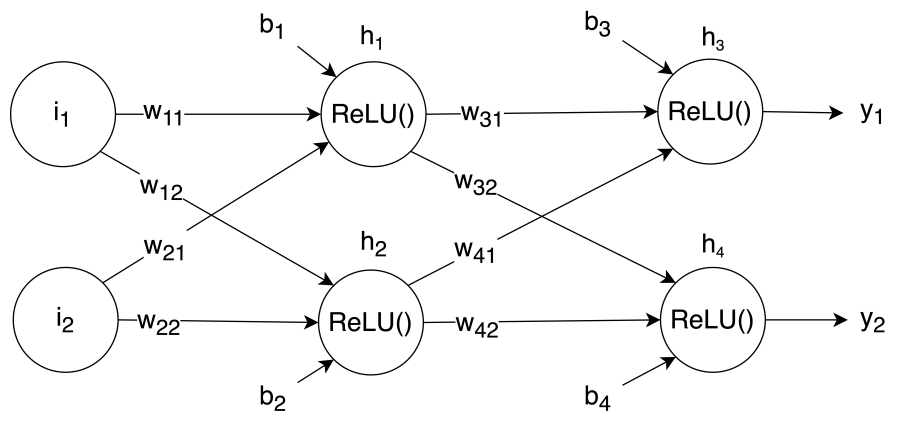
\includegraphics[scale=0.3]{img/nn_example.png} 
    \end{center}
    The values of the variables are given as follows: 
    \begin{table}[H]
      \centering
      \begin{tabular}{|c|c|c|c|c|c|c|c|c|c|c|c|c|c|c|c|}
        \hline
        $i_1$ & $i_2$ & $w_{11}$ & $w_{12}$ & $w_{21}$ & $w_{22}$ & $w_{31}$ & $w_{32}$ & $w_{41}$ & $w_{42}$ & $b_1$ & $b_2$ & $b_3$ & $b_4$ & $t_1$ & $t_2$ \\
        \hline
        1 & 2 & 1 & 0.5 & -0.5 & 1 & 0.5 & -2 & -1 & 0.5 & -0.5 & -0.5 & 1 & 1 & 2 & 4 \\
        \hline
      \end{tabular}
    \end{table}
    \begin{enumerate}
      \item Compute the output $(y_1, y_2)$ of the input $(x_1, x_2)$ using the network parameters as specified above. 
      \item Compute the mean squared error of the computed output and the target labels. 
      \item Using the calculated MSE, update the weight $w_{31}$ using GD with $\eta = 0.01$. 
      \item Do the same with weight $w_{42}$. 
      \item Do the same with weight $w_{22}$.  
    \end{enumerate}
  \end{exercise}

